Here, we provide additional experimental results and analysis. First, we provide a comparison between vanilla baseline methods and results using \qc{} on the baselines on \yoloa{} and \yolob{}. Later, we also provide ablation studies of various setups of \qc{} and show the stability of \exma{} for the decay parameter $(\alpha)$. 

\section{Comparisons with vanilla baselines and \qc{} based baselines}
\begin{table}[h]

\centering
% \vspace{-5ex}
\caption{\em Comparison between \acrshort{LSQ}~\cite{lsq}, Oscillation dampening~\cite{nagel2022overcoming}, and our proposed method after performing our \qc{} for quantization-aware training using mAP metric for object detection task on the \coco dataset.}
\vspace{1ex}
\label{tab:baseline-qc}
\begin{tabular}{lclccc}
\toprule
Method                                 & Ours (\qc{}) & \#-bit                 & \yoloa{-n} & \yoloa{-s} & \yolob{-tiny} \\
\midrule
Full-Precision                         & -         & 32-bit                 & 28.0      & 37.4    & 37.5       \\
\midrule
\multirow{2}{*}{\acrshort{LSQ}~\cite{lsq}}                   & \xmark         & \multirow{6}{*}{4-bit} & 20.6    & 32.4    & 32.9       \\
                                       & \cmark         &                        & 22.6    & 33.3    & 34.1       \\
                                       \cmidrule{4-6}
\multirow{2}{*}{Osc. Dampening~\cite{nagel2022overcoming}} & \xmark         &                        & 21.5    & 32.9    & 33.5       \\
                                       & \cmark         &                        & 23.1    & 33.4    & 34.3       \\
                                       \cmidrule{4-6}
\multirow{2}{*}{Ours (\exma)}            & \xmark         &                        & 22.1    & 33.1    & 34.6       \\
                                       & \cmark         &                        &  \cellcolor{myGray} \textbf{23.8}    & \cellcolor{myGray} \textbf{34.0}      & \cellcolor{myGray} \textbf{35.2}       \\
\midrule
\multirow{2}{*}{\acrshort{LSQ}~\cite{lsq}}                   & \xmark         & \multirow{6}{*}{3-bit} & 15.2    & 27.2    & 28.4       \\
                                       & \cmark         &                        & 17.1    & 29.4    & 30.2       \\
\cmidrule{4-6}
\multirow{2}{*}{Osc. Dampening~\cite{nagel2022overcoming}} & \xmark         &                        & 16.4    & 27.5    & 29.2       \\
                                       & \cmark         &                        & 17.9    & 29.6    & 30.5       \\
                                       \cmidrule{4-6}

\multirow{2}{*}{Ours (\exma)}            & \xmark         &                        & 16.4    & 28.5    & 30.3       \\
                                       & \cmark         &                        & \cellcolor{myGray} \textbf{18.2}    & \cellcolor{myGray} \textbf{30.2}    & \cellcolor{myGray} \textbf{31.0}   \\
\bottomrule
\end{tabular}
\end{table}

Further, we also perform experiments to evaluate the effectiveness of \qc{} on the baseline \acrshort{QAT} methods such as \acrshort{LSQ}~\cite{lsq} and Oscillation dampening~\cite{nagel2022overcoming} on object detection task on \coco{} dataset and the results are reported in \tabref{tab:baseline-qc}. Our \qc{} approach to correct the error induced due to oscillating weights and scale factors cannot only improve the detection performance of quantized models of \exma{} but also the baseline methods. Despite that, our combined approach with both \exma{} and \qc{} outperforms all the baselines with \qc{} consistently at 4-bit as well as 3-bit quantization on \yoloa{} and \yolob{} variants.

\section{Ablation on different \qc{} setups}
\begin{table}[]
\centering
\caption{\em Ablation studies of different \qc{} setups, where either per-tensor or per-channel correction is performed varying whether to use \qc{} scale or shift on \yoloa{-n} trained at 4-bit on \coco{} dataset.}
\vspace{1ex}
\label{tab:qc-ablation}
\begin{tabular}{lccr}
\toprule
\qc{} Setup                     & \qc{} Scale & \qc{} Shift & mAP  \\
\midrule
\multirow{3}{*}{Per-tensor}  & \cmark        & \xmark        & 22.2 \\
                             & \xmark        & \cmark        & 22.3 \\
                             & \cmark        & \cmark        & 22.6 \\
                             \midrule
\multirow{3}{*}{Per-channel} & \cmark        & \xmark        & 23.5 \\
                             & \xmark        & \cmark        & 23.6 \\
                             & \cellcolor{myGray} \cmark        & \cellcolor{myGray} \cmark        & \cellcolor{myGray} \textbf{23.8} \\
\bottomrule
\end{tabular}
\end{table}

\qc{} can correct the error induced due to oscillations after the quantization by employing the per-channel scale and shift correction factors. These scale factors can also be chosen per-tensor. To evaluate the effectiveness of different components of \qc{} such as scale and shift correction factors, we provide ablation studies in \tabref{tab:qc-ablation}. We also provide results on both per-tensor and per-channel setup of \qc{}. It is important to note that both scale and shift parameters are equally important in both per-tensor and per-channel \qc{} setup and neither alone can effectively reduce oscillation-based error. Also, even the simple per-tensor setup of \qc{} improves the \exma{} performance but as expected it cannot meet the performance achieved by the per-channel \qc{} setting.

\section{Effect of varying decay factor in \exma{}}
\begin{table}[]
\centering
\caption{\em Different values of decay parameter $(\alpha)$ in \exma{} for \yoloa{-n} trained at 4-bit on \coco{} dataset. Note, \exma{} is quite stable with respect to different decay parameters. }
\vspace{1ex}
\label{tab:diff-mom-ema}
\begin{tabular}{cr}
\toprule
Decay parameter $(\alpha)$ & mAP  \\
\midrule
0.0              & 20.6 \\
0.9            & 21.5 \\
\cellcolor{myGray} 0.99           & \cellcolor{myGray}\textbf{22.1} \\
\cellcolor{myGray} 0.999          & \cellcolor{myGray} \textbf{22.1} \\
\cellcolor{myGray} 0.9999         & \cellcolor{myGray} \textbf{22.1} \\
\bottomrule
\end{tabular}
\end{table}

To check the stability of \exma{} to varying decay factors, we trained different 4-bit \yoloa{-n} models using \coco{} datasets and the comparisons are provided in \tabref{tab:diff-mom-ema}. As shown, our \exma{} approach is quite stable to different decay parameters. \exma{} takes into into account $\approx1-(1-\alpha)$ iterations to compute the average weights or scale factors. Typically, oscillations are consistent over $\ge100$ iterations, and taking an average of scale factors or weights over $\ge 100$ iterations works effectively in mitigating the oscillation side-effects in the final \acrshort{QAT} model. 

\section{Oscillation in scale factors with or without \exma{}}
To show the effect of \exma{} on the quantization scale factors during the training, we also provide the plots for scale factors during the last 4K iterations of training with or without \exma{} in \figref{fig:scale-wt-yolov5} and \figref{fig:scale-act-yolov5} for scale factors of weights and activations respectively. It can be seen that \exma{} leads to a smoother transition of quantization scale factors for both weights and activations throughout the training and thus lead to stable training of quantized \yolo{} models.
\begin{figure*}[ht]
     \centering
     \begin{subfigure}[b]{0.48\textwidth}
         \centering
         
\includegraphics[width=0.99\textwidth]{figures/appendix/model/wts_stepsize.pdf.pdf}
         \caption{}
         % \label{fig:latent_yolo}
     \end{subfigure}
    %  \hfill
     \begin{subfigure}[b]{0.48\textwidth}
         \centering
         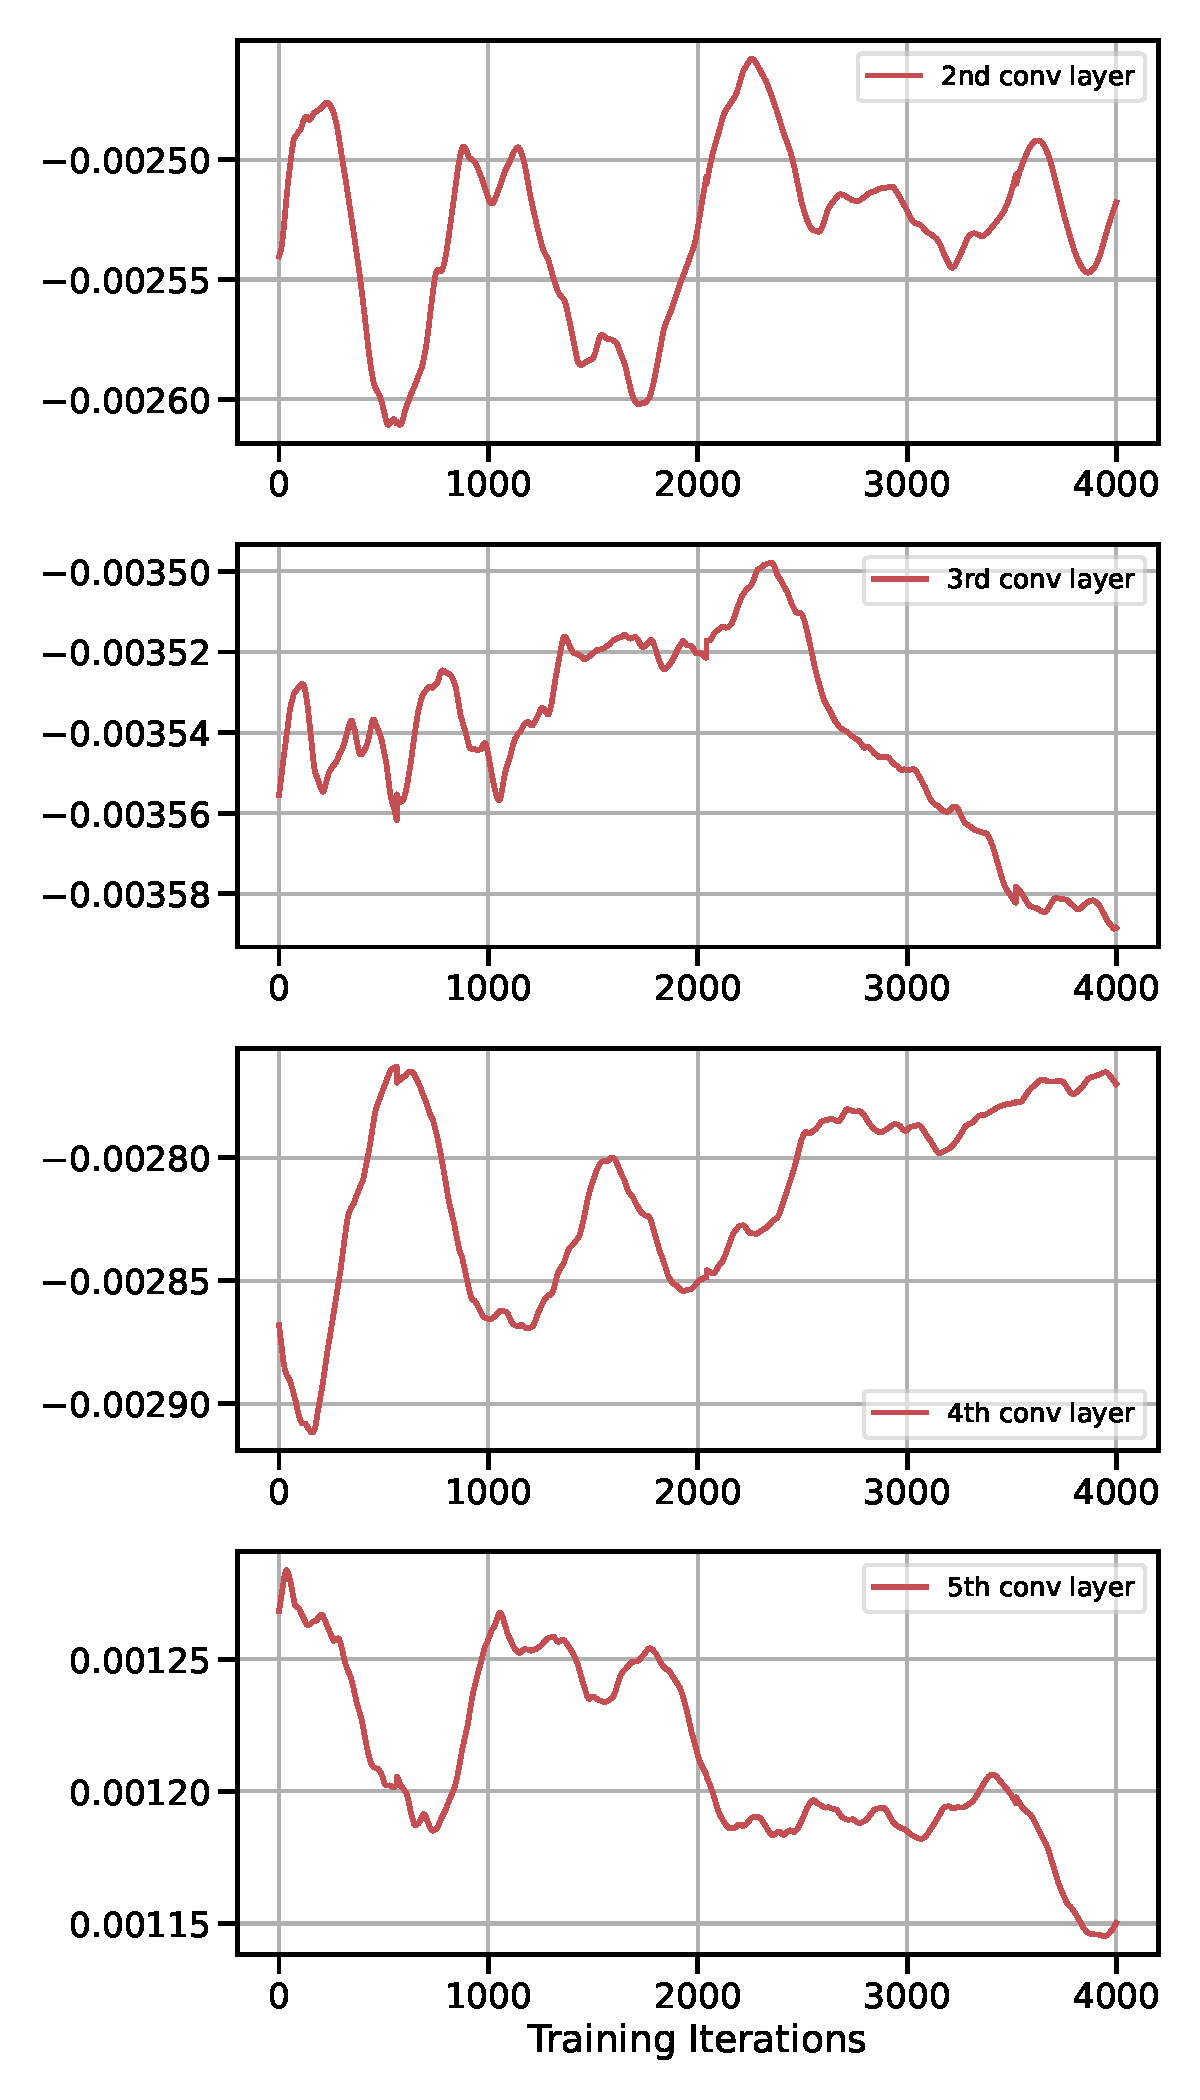
\includegraphics[width=0.99\textwidth]{figures/appendix/ema/wts_stepsize.pdf.pdf}
         \caption{}
         % \label{fig:scalefactor_wt_yolo}
     \end{subfigure}
    % \vspace{-1ex}
        \caption{\em Effect of \exma{} on oscillation issue in \yoloa{}-n variant trained on \coco{} dataset at 4-bit precision using \acrshort{LSQ}~\cite{lsq}. (a) Scale factors for weight quantization in the vanilla model during the last 4K iterations of 2nd-5th conv layer, (b) Scale factors for weight quantization in \exma{} model during the last 4K iterations of 2nd-5th conv layer. Here, it can be observed that \exma{} makes the quantization scale factors stable for all the layers and gets rid of the oscillation issue.}
        \label{fig:scale-wt-yolov5}
    % \vspace{-3ex}
\end{figure*}

\begin{figure*}[ht]
     \centering
     \begin{subfigure}[b]{0.48\textwidth}
         \centering
         
\includegraphics[width=0.99\textwidth]{figures/appendix/model/acts_stepsize.pdf.pdf}
         \caption{}
         % \label{fig:latent_yolo}
     \end{subfigure}
    %  \hfill
     \begin{subfigure}[b]{0.48\textwidth}
         \centering
         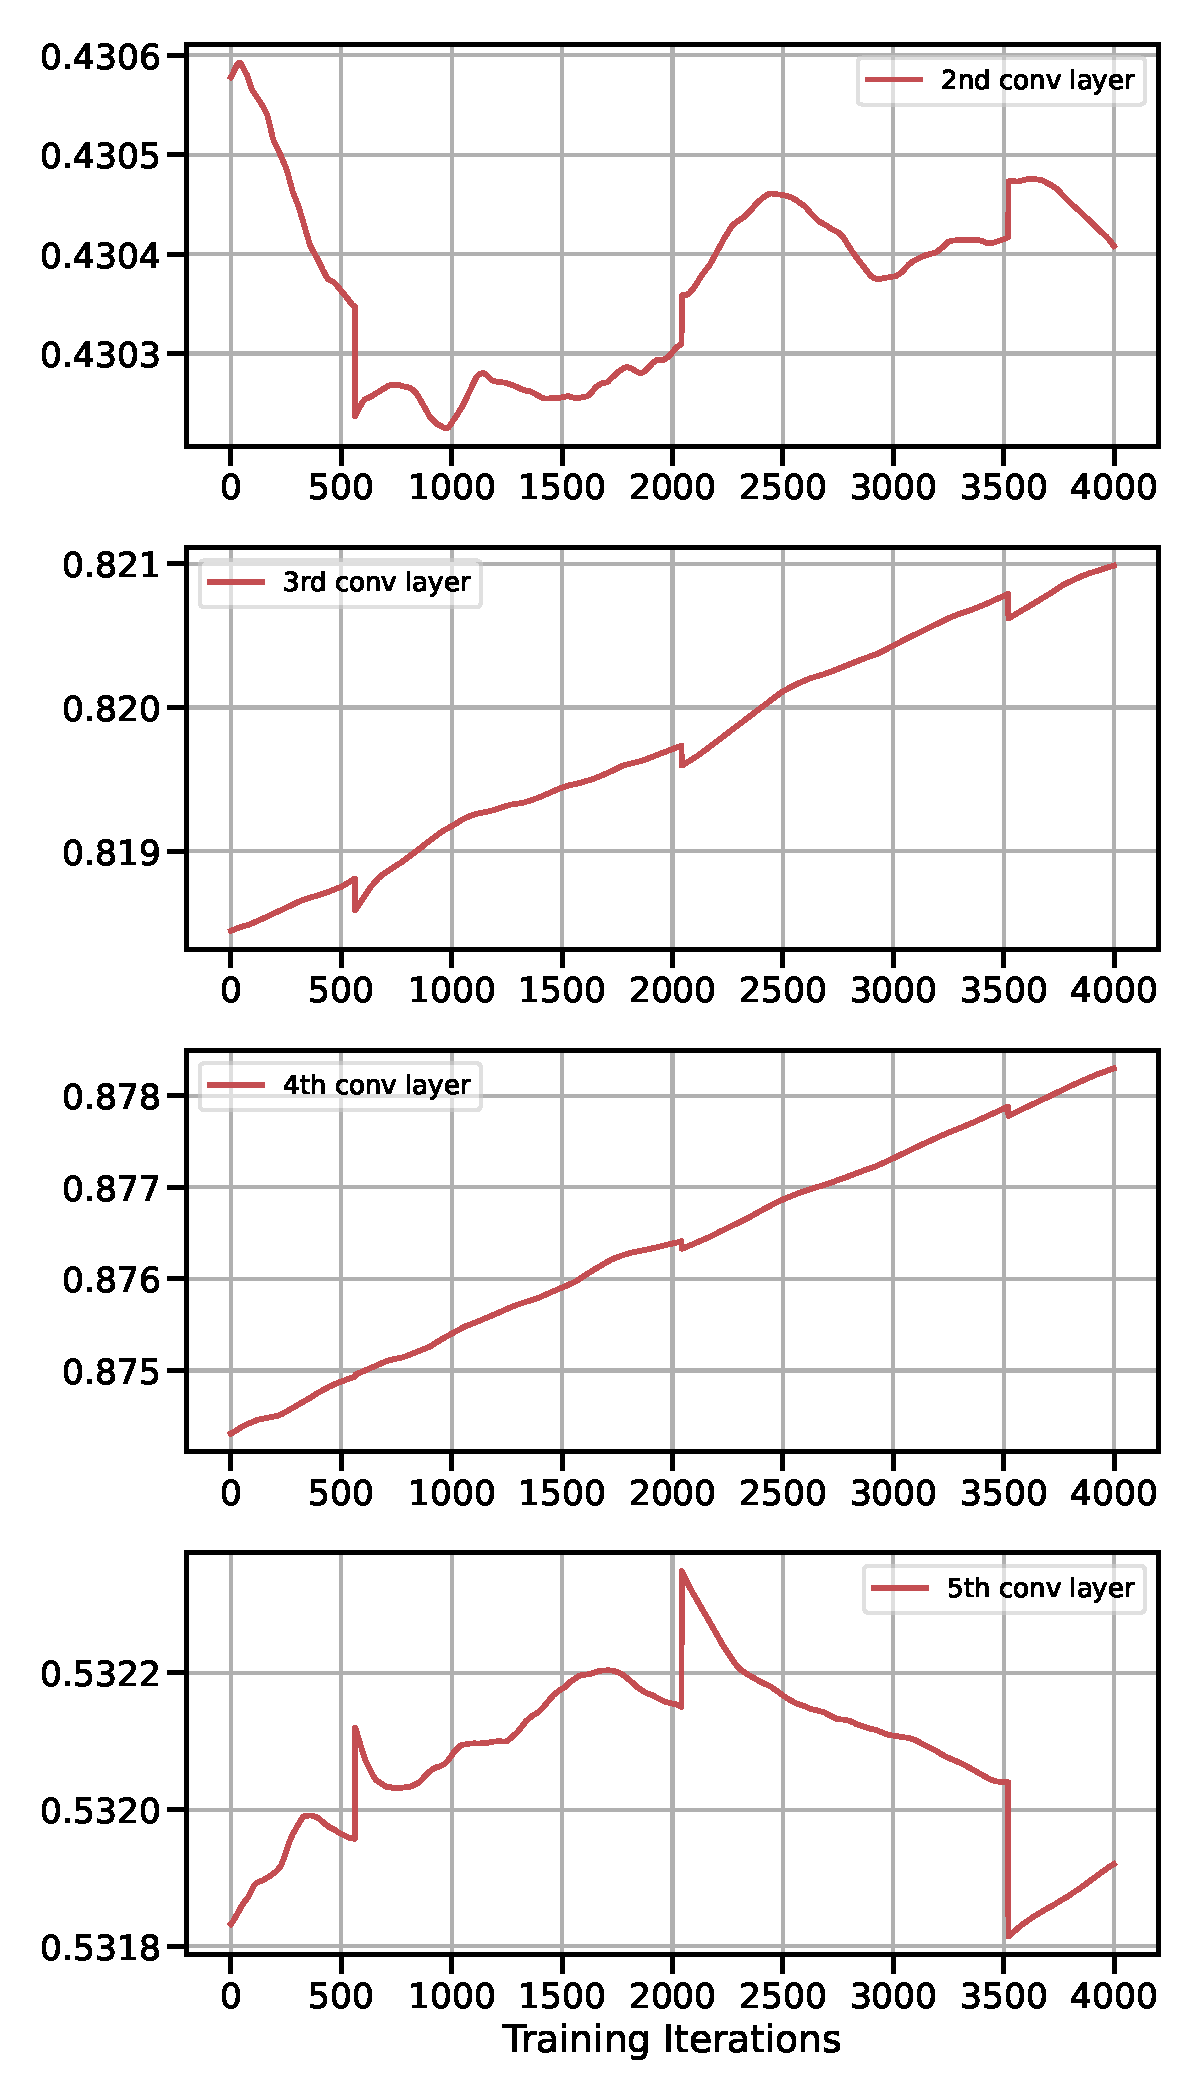
\includegraphics[width=0.99\textwidth]{figures/appendix/ema/acts_stepsize.pdf.pdf}
         \caption{}
         % \label{fig:scalefactor_act_yolo}
     \end{subfigure}
    % \vspace{-1ex}
        \caption{\em Effect of \exma{} on oscillation issue in \yoloa{}-n variant trained on \coco{} dataset at 4-bit precision using \acrshort{LSQ}~\cite{lsq}. (a) Scale factors for activation quantization in the vanilla model during the last 4K iterations of 2nd-5th conv layer, (b) Scale factors for activation quantization in \exma{} model during the last 4K iterations of 2nd-5th conv layer. Here, it can be observed that \exma{} makes the quantization scale factors stable for all the layers and gets rid of the oscillation issue.}
        \label{fig:scale-act-yolov5}
    % \vspace{-3ex}
\end{figure*}




 

